\section{解答题：本题共 5 小题，共 70 分。解答应写出文字说明、证明过程或演算步骤。}

% 15.
\begin{problem}[points = 10]
  四棱台的上下底面边长分别为 $2$ 和 $4$, 侧棱长为 $4$.
  \begin{enumerate}
    \item 求它的表面积;
    \item 求它的体积.
  \end{enumerate}
\end{problem}

% 16.
\begin{problem}[points = 12]
  已知向量 $\overrightarrow{OA}=(1,1)$, $\overrightarrow{OB}=(3,-1)$, $\overrightarrow{OC}=(m,3)$, $\overrightarrow{OD}=(x,y)$, 其中 $O$ 为坐标原点．
  \begin{enumerate}
    \item 若 $A,B,C$ 三点共线, 求实数 $m$ 的值;
    \item 当四边形 $ABCD$ 为矩形时, 设点 $M$ 为线段 $CD$ 的中点, 问在线段 $AD$ 上是否存在点 $N$ 使得 $|\overrightarrow{NB}+\overrightarrow{NM}|=\dfrac{\sqrt{194}}{3}$, 若存在, 请求出所有满足条件的点 $N$ 的坐标, 若不存在, 说明理由．
  \end{enumerate}
\end{problem}

% 17.
\textfigure[fig-pos=bottom-flushright]{
  \begin{problem}[points = 12]
    “我将来要当一名麦田里的守望者, 有那么一群孩子在一块麦田里玩, 几千万的小孩子, 附近没有一个大人,我是说……除了我”《麦田里的守望者》中的主人公霍尔顿将自己的精神生活寄托于那广阔无垠的麦田. 假设霍尔顿在一块成凸四边形$ABCD$的麦田里成为守望者. 如图所示,为了分割麦田, 他将$BD$连接, 设$\triangle ABD$中边$BD$所对的角为$A$, $\triangle BCD$中边BD所对的角为$C$. 经测量知$AB = BC = CD = 2, AD = 2\sqrt{3}$.
    \begin{enumerate}
      \item 若$A = 30^\circ$, 求$C$;
      \item 霍尔顿发现无论$BD$多长, $\sqrt{3}\cos A - \cos C$为一个定值. 请你验证霍尔顿的结论, 并求出这个定值.
      \item 霍尔顿发现麦田的的生长与土地面积的平方呈正相关, 记$\triangle ABD$与$\triangle BCD$ 的面积分别为$S_1$和$S_2$, 为了更好地规划麦田, 请你帮助霍尔顿求出$S_1^2 + S_2^2$的最大值.
    \end{enumerate}
  \end{problem}
}{
  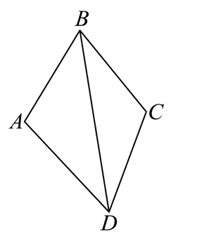
\includegraphics[width=3cm]{figure/17.png}
}

% 18.
\begin{problem}[points = 12]
  \textfigure[fig-pos=bottom-center]{
    矩形$ABCD$中, $AB = 2AD = 2$, $P$为线段$DC$的中点. 将$\triangle ADP$沿着$AP$折起, 使得平面$ADP\perp$平面$ABCP$. 在新构造的四棱锥$D-PABC$中, 求解以下问题:
    \begin{enumerate}
      \item 求四棱锥$D-PABC$的体积.
      \item 求二面角$P-AD-B$的余弦值.
      \item 在$DC$上是否存在点$E$使得$AD\parallel$平面$PBE$? 若存在, 求出点$E$的位置; 若不存在, 请说明理由.
    \end{enumerate}
  }{
    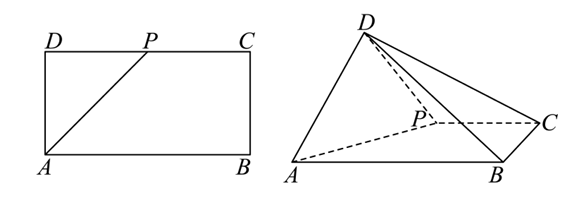
\includegraphics[width = 12cm]{figure/18.png}
  }
\end{problem}

% 19.
\begin{problem}[points = 12]
  已知$s$是直线$PQ$外一点, 点$M, N$在直线$PQ$上.（点$M, N$与点$P, Q$任一点均不重合）我们称如下操作为“由$s$点对$PQ$施以视角运算”:
  \begin{itemize}
    \item 若点$M$在线段$PQ$上, 记$(P, Q; M) = \frac{\left|SP\right|\sin\angle PSM}{\left|SQ\right|\sin\angle MSQ}$; 
    \item 若点$M$在线段$PQ$外, 记$(P, Q; M) = -\frac{\left|SP\right|\sin\angle PSM}{\left|SQ\right|\sin\angle MSQ}$.
  \end{itemize}
  并且记$(P, Q; M, N) = \frac{(P, Q; M)}{(P, Q; N)}$. 记$\triangle ABC$的内角$A, B, C$的对边分别为$a, b, c$. 已知$b=2$, $A = 60^\circ$, $D$是射线$BC$上的一点. 现由$A$点对$BC$施以视角运算, 得到$(B, C; D) = \frac{c}{2}$.
  \begin{enumerate}
    \item 若$\left|AD\right| = \sqrt{3} + 1$, 求$\overrightarrow{AD}\cdot\overrightarrow{DC}$的值;
    \item 射线$BC$上的点$M$满足$(B, C; M, D) = -2$.
    \begin{enumerate}
      \item 求$\angle CAM$;
      \item 求$\left|AM\right| + 16\left|AD\right|$的最小值.
    \end{enumerate}
  \end{enumerate}

  \begin{solution}
    函数的定义域为 $(0, +\infty)$,
    又 \[f^{\prime}(x) = 1 - \ln x-1 = -\ln x, \score{2}\]
    当 $x \in(0, 1)$ 时, $f^{\prime}(x) > 0$, 当 $x \in(1, +\infty)$ 时, $f^{\prime}(x) < 0$,
    故 $f(x)$ 的递增区间为 $(0,1)$, 递减区间为 $(1, +\infty)$.
  \end{solution}
\end{problem}
